\chapter{SPI sučelje i DMA prijenos}

SPI protokol se koristi za prijenos podataka između \textit{flash} memorije i mikrokontrolera, odnosno međuspremnika kamere. Kako bi se oslobodili resursi na mikrokontroleru, za prijenos podataka između kamere i \textit{flash} memorije se, u kombinaciji s SPI protokolom, koristi i DMA prijenos. S obzirom da se koriste \textit{Low-Layer} biblioteke, potrebno je razumijeti način rada SPI i DMA periferija mikrokontrolera. U ovom poglavlju biti će opisan SPI protokol i DMA prijenos i biti će istaknute razlike i problemi kod prilagođavanja programske podrške na STM32L471VGT6 mikrokontroler.

\section{SPI protokol}

SPI (engl. \textit{Serial Peripheral Interface} je sinkrono serijsko komunikacijsko sučelje koje se koristi za komunikaciju na kratkim udaljenostima, pretežito u ugradbenim računalnim sustavima \cite{spi_wikipedia}. 

SPI uređaji komuniciraju u \textit{full-duplex} načinu rada koristeći \textit{master-slave} arhitekturu, obično sa jednim \textit{master} uređajem. \textit{Master} (upravljač) uređaj proizvodi okvir za čitanje i pisanje. Više \textit{slave} uređaja može biti spojeno na jedan upravljač tako da se aktivira određeni \textit{chip select} signal za pojedini uređaj.

\subsection{Opis sučelja}

SPI sabirnica se sastoji od četiri signala:
\begin{itemize}
	\item SCLK: Serijski takt (izvor je \textit{master} uređaj)
	\item MOSI: \textit{Master Output Slave Input} (izvor podataka iz \textit{master} uređaja)
	\item MISO: \textit{Master Input Slave Output} (izvor podataka iz \textit{slave} uređaja)
	\item CS/SS: \textit{Chip/Slave Select} (aktivan nisko, signal iz \textit{master} uređaja, označava da se prenose podaci)
\end{itemize}
MOSI na \textit{master} uređaju se spaja na MOSI na \textit{slave} uređaju, dok se MISO na \textit{master} uređaju se spaja na MISO na \textit{slave} uređaju. CS/SS se koristi za pokretanje komunikacije između \textit{slave} i \textit{master} uređaja. Za svaki \textit{slave} uređaj postoji zaseban CS/SS priključak na \textit{master} uređaju. Primjer spajanja tri \textit{slave} uređaja na jedan \textit{master} uređaj prikazan je na slici \ref{fig:spi_three_slaves}.
\begin{figure}[H]
	\centering
	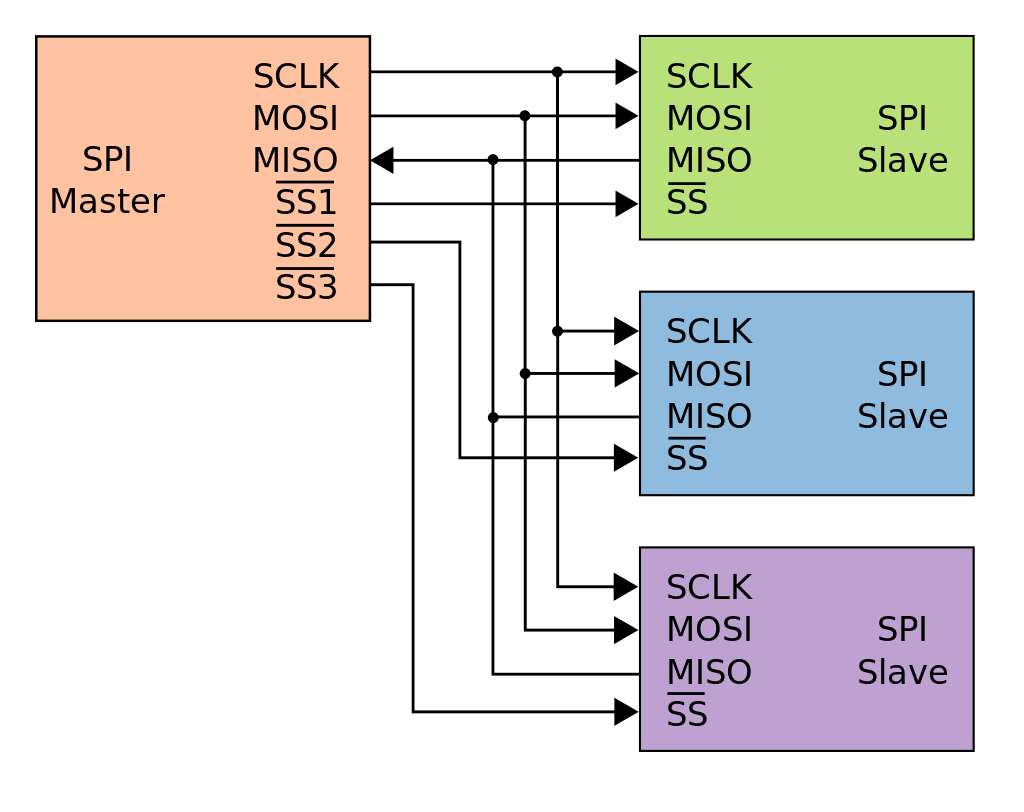
\includegraphics[height=7 cm]{SPI_three_slaves.svg.png}
	\caption{Spoj tri \textit{slave} uređaja na jedan \textit{master} uređaj. Vidljivo je da \textit{master} uređaj ima tri SS priključka, a svaki odgovara jednom \textit{slave} uređaju, dok se SCLK, MOSI i MISO linije međusobno dijele između \textit{slave} uređaja \cite{spi_wikipedia}}
	\label{fig:spi_three_slaves}
\end{figure}

\subsection{Način rada}

SPI sabirnica radi sa jednim \textit{master} uređajem i jednim ili više \textit{slave} uređaja. Ako se koristi jedan \textit{slave} uređaj, onda CS stezaljka može biti cijelo vrijeme postavljena u niskom logičkom stanju, ako \textit{slave} uređaj to dopušta. Neki \textit{slave} uređaji zahtijevaju padajući brid CS signala kako bi započeča komunikacija. Ako se koristi više \textit{slave} uređaja potreban je zaseban CS signal \textit{master} uređaja za svaki \textit{slave} uređaj.

\subsubsection{Prijenos podataka}

Za početak komunikacije \textit{master} uređaj konfigurira takt koristeći frekvenciju koju podržava \textit{slave} uređaj, obično do nekoliko \si{MHz}. \textit{Master} uređaj zatim odabire \textit{slave} uređaj postavljanjem CS linije u nisko logičko stanje. Ako je potreban period čekanja, npr. za ADC konverziju, \textit{master} uređaj mora pričekati minimalno taj period vremena prije puštanja takta.

Tijekom svakog perioda takta obavlja se prijenos podataka u \textit{full-duplex} načinu prijenosa. To znači da \textit{master} uređaj pošalje jedan bit na MOSI liniju, kojega \textit{slave} uređaj pročita, dok u isto vrijeme \textit{slave} uređaj šalje jedan bit na MISO liniju, kojega \textit{master} uređaj pročita. Takva sekvenca se održava čak i kada se izvađa jednosmjeran prijenos podataka.

Prijenosi podataka uključuju dva posmačna registra zadane veličine, npr. 8 bitova, jedan u \textit{master} i drugi u \textit{slave} uređaju. Registri su spojeni u topologiji virtualnog prstena (slika \ref{fig:spi_circular_transfer}).
\begin{figure}[H]
	\centering
	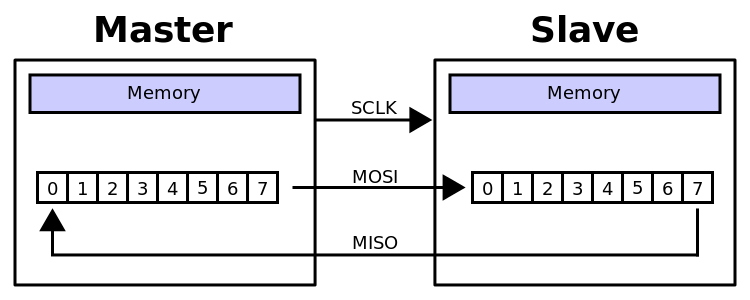
\includegraphics[width=\textwidth]{SPI_8-bit_circular_transfer.svg.png}
	\caption{Tipičan spoj dvaju posmačna registra koji formiraju kružni međuspremnik \cite{spi_wikipedia}}
	\label{fig:spi_circular_transfer}
\end{figure}
Podaci se obično pomiču na način da se prvo pomakne najznačajniji bit. Na brid takta, \textit{master} i \textit{slave} uređaj pomaknu bit i pošalju ga na prijenosnu liniju. Na sljedeći brid takta, na svakom prijamniku bit se uzorkuje sa prijenosne linije i postavlja se kao novi najmanje značajni bit u posmačnom registru. \textit{Master} i \textit{slave} uređaji u potpunosti razmjene podatke u registrima nakon što se svi bitovi u registrima prebace. Ako je potrebno razmjeniti još podataka, posmačni registri se ponovno napune te se postupak ponavlja, a prijenos se može obavljati za bilo koji broj perioda takta. Kada je prijenos dovršen, \textit{master} uređaj prestaje davati takt i obično isključi CS signal, odnosno postavi ga na visoku razinu.

Prijenos se obično obavlja u širinama podataka od 8 bitova, no moguć je i 16 bitni prijenos, ili čak 12 bitni prijenos, koji se koristi za DAC i ADC konvertere.